%% LyX 2.3.6 created this file.  For more info, see http://www.lyx.org/.
%% Do not edit unless you really know what you are doing.
\documentclass[11pt,english]{article}
\usepackage{mathptmx}
\usepackage{helvet}
\usepackage{courier}
\usepackage[T1]{fontenc}
\usepackage[latin9]{inputenc}
\usepackage[a4paper]{geometry}
\geometry{verbose,tmargin=1cm,bmargin=2cm,lmargin=2cm,rmargin=2cm}
\usepackage{babel}
\usepackage{array}
\usepackage{multirow}
\usepackage{graphicx}
\usepackage{setspace}
\onehalfspacing
\usepackage[unicode=true,pdfusetitle,
 bookmarks=true,bookmarksnumbered=false,bookmarksopen=false,
 breaklinks=false,pdfborder={0 0 1},backref=false,colorlinks=false]
 {hyperref}

\makeatletter

%%%%%%%%%%%%%%%%%%%%%%%%%%%%%% LyX specific LaTeX commands.
%% Because html converters don't know tabularnewline
\providecommand{\tabularnewline}{\\}
%% A simple dot to overcome graphicx limitations
\newcommand{\lyxdot}{.}


%%%%%%%%%%%%%%%%%%%%%%%%%%%%%% Textclass specific LaTeX commands.
\newenvironment{lyxcode}
	{\par\begin{list}{}{
		\setlength{\rightmargin}{\leftmargin}
		\setlength{\listparindent}{0pt}% needed for AMS classes
		\raggedright
		\setlength{\itemsep}{0pt}
		\setlength{\parsep}{0pt}
		\normalfont\ttfamily}%
	 \item[]}
	{\end{list}}

%%%%%%%%%%%%%%%%%%%%%%%%%%%%%% User specified LaTeX commands.
\date{}

\makeatother

\begin{document}
\title{LaRVa\\
Last ``Another RISC-v'' from VAlladolid}
\author{J. Arias}
\maketitle

\section{Introduction}

LaRVa is a minimal RV32E/RV32I core designed with three goals in mind:
\begin{enumerate}
\item It has to be simple, easy to understand, and to fit into small FPGAs.
\item It has to run fast.
\item It has to support vectored interrupts.
\end{enumerate}
Goal \#1 was dictated by the FPGAs we are using in lots of designs:
the ICE40HX family from Lattice, and also by common sense.

Goal \#2 implies a pipelined execution, something I explored with
success in the design of the GUS16 processor, and that most simple
RV cores, like ``PicoRV'' from Claire Wolf, or ``FemtoRV'' from
Bruno Levy \& Matthias Koch, lack. laRVa is going to execute one instruction
each clock cycle, unless these instructions are loads, stores, or
jumps.

Goal \#3 demands some way to save the value of the PC when an interrupt
is serviced. I resorted to use two different PC registers, one for
normal mode and other for interrupts, so there is no need to save
anything. 

Why to design another CPU core? Well, the GUS16 was a successful design,
but with a very big problem: It has no GCC toolchain! Its only tool
is a lousy 2-pass assembler and that's all folks. Apart from that
it is a 16-bit design with many limitations. On the contrary, the
RISC-V have a powerful toolchain maintained by GNU and it is a 32-bit
design.

Of course, this design is going to present some challenges apart from
the fact that it uses double the number of bits than the GUS16, like:
\begin{itemize}
\item A big register bank that can't be mapped to internal RAM blocks (BRAMS).
The problem with BRAMS is their synchronous read, or the fact that
the data you are reading isn't available until next clock edge, a
time I don't want to waste. 32 registers of 32 bits each will require
no less than 1024 flip-flops or logic cells, so a 16-register approach
(RV32E) could be a good idea to start with. 
\item A lot of sign extensions are needed for literals and also for the
bytes and half-words read from memory. And, in some cases zero extensions.
\item The usual ALU has to be complemented with a barrel shifter in order
to support single cycle multi-bit shifts.
\item The ``Set Less Than'' instructions also have to be supported in
the ALU.
\item Conditional branches do use the ALU for the checking of conditions
(there are no comparisons, nor condition flags here), but they also
require the addition of an literal offset to PC, thus, a second adder
has to be included for the PC update during jumps.
\item Talking about PC offsets. In the RISC-V ISA all offsets are related
to the address of the current instruction, but in a pipelined processor
the PC is going to point ahead of the instruction being executed.
This fact has to be taken into account in the processor design (not
in the assembler like in the GUS16 case, or ARM's, or many others)
\item While the RISC-V ISA is very clear and concise about its base integer
instructions, when it comes to privileged mode it becomes just the
contrary. I'm not going to waste a single logic cell for the implementation
of a ``Vendor ID'' register, profiling register, or any crap like
that. I just want a minimally decent implementation of hardware interrupts,
so, the only register I'm planning to implement is the ``MEPC''
(Machine Exception PC) along with the ``MRET'' instruction for copying
it back to PC or something equivalent like the use of two PC registers.
\end{itemize}

\section{LaRVa design}

This processor follows a pipelined execution where two instructions
are processed in parallel: One gets its op-code read from memory and
the other gets executed. An Instruction register holds the op-code
while a new one is being read, and all instructions must complete
their execution in a single cycle. This last requirement leaves out
the multiplication and division instructions and forces the use of
a barrel shifter in the ALU, along with ruling out the use of BRAM
blocks with synchronous outputs for the synthesis or the register
file. 

Also, not all instructions can be executed in this way: Load and Store
operations have to address the memory during their execution cycle,
and therefore, no op-code fetch can be carried out simultaneously.
In this case an invalid op-code is stored in the instruction register
and it has to be signaled and discarded. This results in the use of
two effective clock cycles for the execution of Load or Store instructions.
Something similar happens during jumps, where the op-code read into
the instruction register is the one at the memory position following
the jump instruction, and that instruction shouldn't be executed.
In the case of jumps two effective cycles are also employed, and conditional
jumps will take two cycles if their condition is meet or just one
cycle otherwise.

Apart from these details, the design of the LaRVa core is quite conventional
with three data buses: two inputs and one output to the ALU. A good
deal of Verilog code was taken from the ``FemtoRV'' sources, specially
that related to the ALU design or the Load/Store management. Some
of this code remains almost untouched, like the mentioned Load/Store
logic, while other was heavily modified, like the ALU. And, of course,
some other code is completely new, like the register file, the the
program counter stack (LaRVa has two PCs), and the interrupt logic,
that was almost literally copied from the GUS16 design.

With respect to the FemtoRV design I want to remark the following
changes:
\begin{itemize}
\item The ALU is now used for the computation of memory addresses during
the execution of Load and Store instructions. The address bus is switched
from the PC to the output of the ALU adder during these instructions.
\item The ALU is also used for the computation of the jumping address for
the JALR instruction, and the results of the AUIPC and LUI instructions.
\item There are no separate adder and subtractor circuits in the ALU. These
two blocks were merged.
\end{itemize}

\subsection{General diagram}

A general view of the design is presented in the following diagram:
\begin{center}
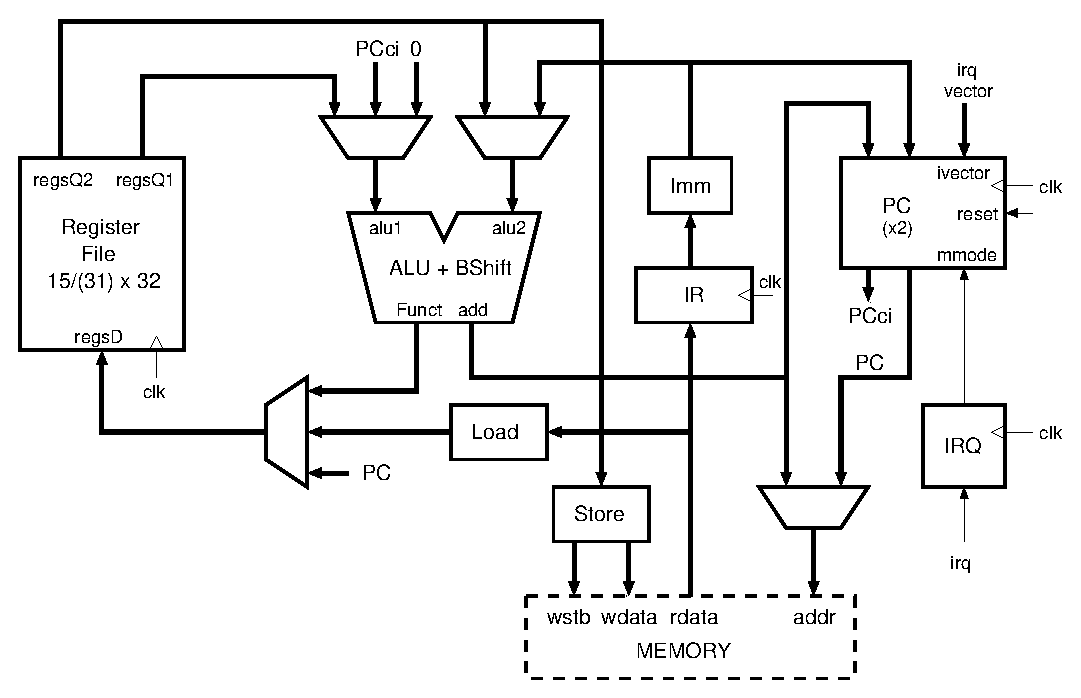
\includegraphics[width=0.9\columnwidth]{larvablk}
\par\end{center}

Here, most blocks are combinational and they are controlled by the
bits stored in the IR register, that holds the op-code of the instruction
being executed. IR also holds the bits of the immediate values that
are further processed in the Imm block, mainly for bit descrambling
and sign extension. 

The ALU includes mainly an adder and a barrel shifter. In its output
the desired operation (ADD, SUB, AND, OR, XOR, Shifts,...) can be
selected, but the outpuPicoRVt of the adder is also always present.
This second output is used for the generation of the memory address
during Load and Store instructions, and also by the JALR instruction
(in fact, the main output of the ALU could also be used, but it has
a little longer delay). The first ALU input is usually the contents
of the register ``rs1'', but it can be also the delayed PC for the
AUIPC instruction or even zero for the LUI instruction. The second
ALU input is selected between the register ``rs2'' or an immediate
constant

The value written back to the register file (register ``rd'') is
the output of the ALU for most cases, a value derived from the data
coming from memory for Load instructions, or the current value of
the program counter (address of next instruction) for the JAL and
JALR instructions. No value is written back in the case of Store,
Branch, or System instructions, or in the case of invalid values in
IR (pipeline stalls).

The program counter block will be described in detail later. Here
I want to remark that it is actually a two-level stack that resembles
the case of 8-bit PIC microcontrollers. One of its registers is used
during normal program execution, while the other is switched in when
an interrupt happens. The normal PC remains unchanged during the execution
of interrupt routines and it is switched back when a return from interrupt
(MRET) is executed. Also, while in normal mode, the interrupt PC gets
preloaded with a vector that could be made different for each possible
interrupt source.

The only remaining block is the one related to interrupt management,
that will be detailed later.

\subsection{Program counter}

A more detailed diagram of the Program Counter logic is shown next:
\begin{center}
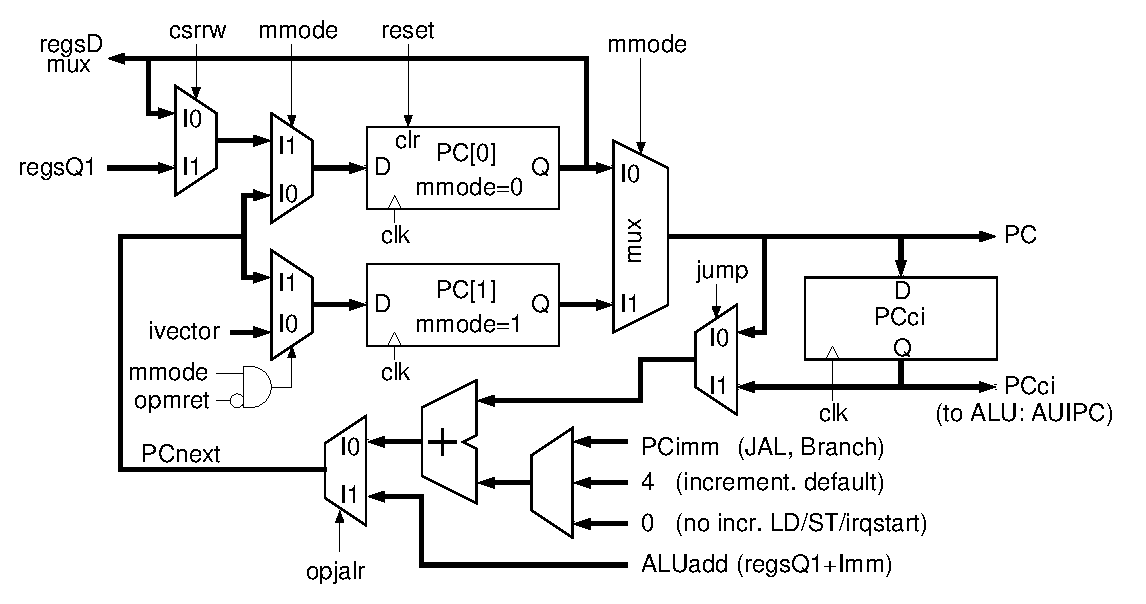
\includegraphics[width=0.7\columnwidth]{PCdual}
\par\end{center}

The ``mmode'' signal selects which register to present at the output,
and also the values written back to each register. In normal mode
(mmode=0) the register PC{[}0{]} is selected as output and it is updated
every clock cycle, while the register PC{[}1{]} is written with the
value ``ivector'', that is the address of the next interrupt service
routine. In interrupt (AKA machine) mode PC{[}0{]} remains with it
last value stored and PC{[}1{]} is presented at the output and updated.

The update logic is built around an adder that allows the PC incrementing
(as op-codes are 32-bit long the PC increments in steps of 4), the
addition of offsets for the execution of conditional branches and
also the JAL instruction, or to leave the PC as it is (increment of
0), that is also required during the execution of Load and Store instructions,
or when the mode changes to interrupt. The JALR instruction is an
special case because the jumping address is computed in the ALU (the
base register is one of the register file, not the PC), and the ALU
output has to be switched in during the execution of JALR.

The AND gate that controls the writing of PC{[}1{]} is intended for
the chaining of interrupts, and it forces the writing of ``ivector'',
even in interrupt mode, when the MRET instruction is executed.

There is also another register (``PCcurInst'', not shown) where
the PC value is copied, so, it has the same value as the PC but with
a one cycle delay. This register holds the address of the instruction
currently being executed and its contents are used for the computation
of branch and JAL address, and for the AUIPC instruction. (I think
a register is cheaper and faster than an adder for the subtraction
of 4).

I want to notice that during interrupt mode the register PC{[}0{]}
is acting as an effective MEPC (Machine Exception PC) and it would
be interesting to be able to read and to modify it. That would provide
support for task switching. In order to have a minimally compliant
implementation of the related privileged ISA the CSRRW instruction
was also added to the core instruction set, yet restricted to its
use with the control/status register \#0x341 (MEPC). This instruction
allows the atomic read plus write of the MEPC register, that is in
fact PC{[}0{]}.

So, now we have two privileged instructions that can be used only
in machine mode. If they are executed in the normal user mode they
will fail for sure. There instructions are:
\begin{enumerate}
\item MRET. When executed in machine mode returns to user mode and restores
the original PC (if there are no interrupts still pending) returning
to the interrupted program. If executed in user mode it does nothing.
\item CSRRW rd,0x341,rs1. When executed in machine mode copies the value
of PC{[}0{]} (MEPC) to ``rd'' and the value of ``rs1'' to PC{[}0{]}.
No other offsets in the CSR space are allowed. If executed in user
mode PC{[}0{]} isn't written, but in ``rd'' we get the current value
of PC.
\end{enumerate}

\subsection{Interrupts}

The servicing of an interrupt implies the changing of the ``mmode''
signal to 1, but this has to be done in a proper sequence in order
to avoid disturbing the instruction being executed. That instruction
has to complete its execution cycle with the normal PC still selected.
In order to achieve this an ``irqstart'' signal is set during just
one clock cycle, and this signal will cause a pipeline stall just
before the change of ``mmode''. 

The details of such sequencing are shown in the next chronograph:
\begin{center}
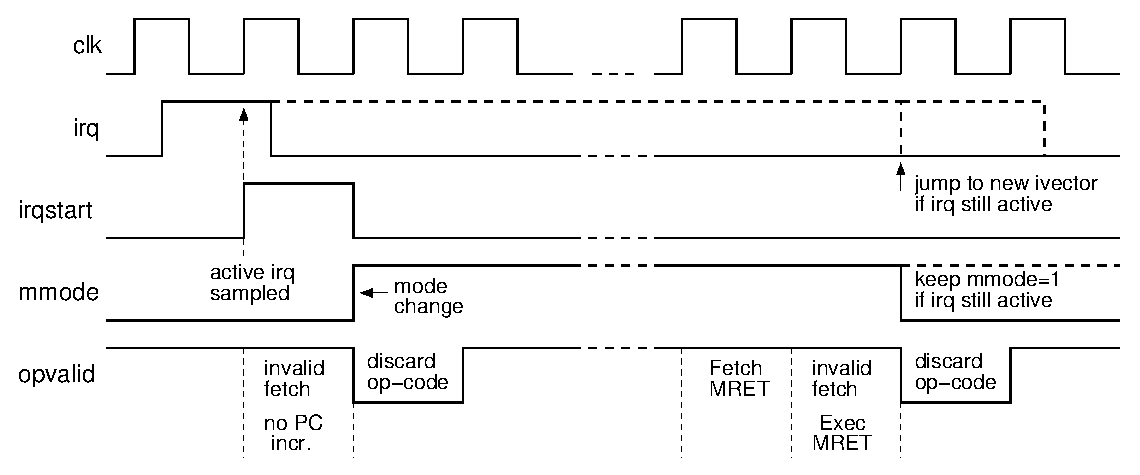
\includegraphics[width=0.9\columnwidth]{IRQcrono}
\par\end{center}

Also, at the end of the interrupt routine an MRET instruction is executed.
That instruction usually returns ``mmode'' to 0 and causes a pipeline
stall, but, if the ``irq'' line is still active ``mmode'' remains
at 1 and interrupts are thus chained.

The circuit diagram for the interrupt sequencing is shown next. It
is the same as in the GUS16 core:
\begin{center}
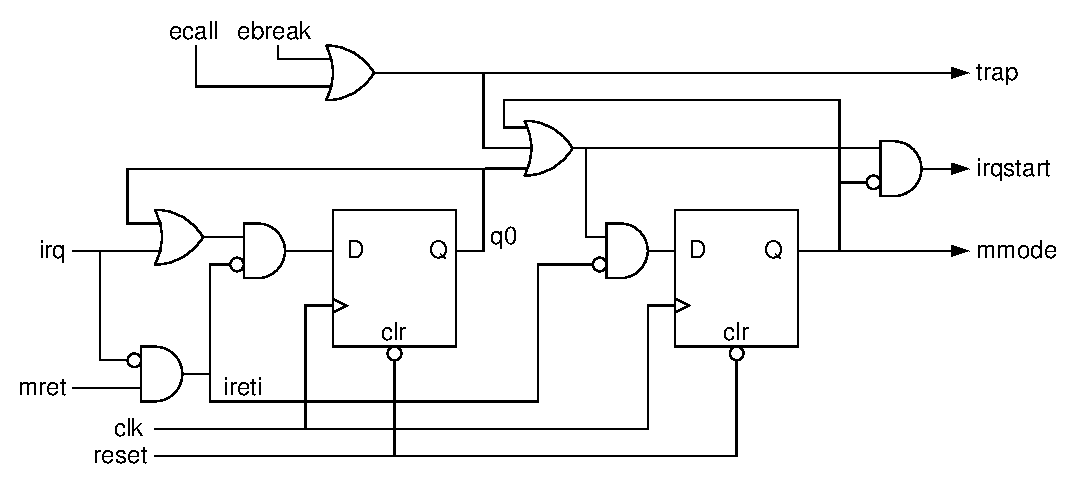
\includegraphics[width=0.7\columnwidth]{IRQlogic}
\par\end{center}

There was also a need for some sort of ``software interrupt'', so,
the ECALL and EBREAK opcodes were also decoded and they act in a similar
way to the ``irqstart'' signal, entering the interrupt mode. But
I didn't want to provide a particular interrupt vector for these opcodes,
so, I resorted to provide a ``trap'' output for the core that can
be routed to an external vectored interrupt controller just like any
other interrupt from a peripheral. 

\subsection{Memory interface \& Wait States}

The LaRVa core has a simple memory interface, including:
\begin{itemize}
\item ``{[}31:2{]}addr'', the memory address. It lacks the two lower bits
because these address are for bytes and the data bus is 32-bit wide.
\item ``{[}31:0{]}rdata'', the data read from the memory/IO system. Its
has 32 bits, but for byte and half-word loads some of these bits are
ignored. 
\item ``{[}31:0{]}wdata'', the data to write to the memory/IO system.
For byte and half-word stores some of these bits are invalid and shouldn't
be written (see write strobes next).
\item ``{[}3:0{]}wstrb'', the four write strobes:
\end{itemize}
\begin{center}
\begin{tabular}{|c|c|c|}
\hline 
wstrb & bits to write & Instruction\tabularnewline
\hline 
\hline 
0001 & wdata{[}7:0{]} & \multirow{4}{*}{SB}\tabularnewline
\cline{1-2} \cline{2-2} 
0010 & wdata{[}15:8{]} & \tabularnewline
\cline{1-2} \cline{2-2} 
0100 & wdata{[}23:16{]} & \tabularnewline
\cline{1-2} \cline{2-2} 
1000 & wdata{[}31:24{]} & \tabularnewline
\hline 
0011 & wdata{[}15:0{]} & \multirow{2}{*}{SH}\tabularnewline
\cline{1-2} \cline{2-2} 
1100 & wdata{[}31:16{]} & \tabularnewline
\hline 
1111 & wdata{[}31:0{]} & SW\tabularnewline
\hline 
\end{tabular}
\par\end{center}

I want to remark that ``addr'' changes after each rising edge of
``clk'' and ``rdata'' must be valid before the next rising edge.
Or in other words: The memory is supposed to be an asynchronous one.
If this core is to be interfaced to a synchronous RAM, like that found
inside FPGAs, it's a good idea to use an inverted clock for the memory.
That would change the RAM output on the falling edges, half a cycle
before its sampling by the core.

With respect to other cores, like PicoRV or FemtoRV, there are two
control lines missing:
\begin{itemize}
\item ``mem\_valid'' output. The LaRVa core is reading or writing the
memory all the clock cycles, so, a ``mem\_valid'' signal would be
always active.
\item ``mem\_ready'' input. There is no control input to force the insertion
of wait states in the core. This may difficult the interfacing of
slow memory devices, like the ``SPI\_flash\_as\_ROM'' ones, or other
memory-master devices like video controllers or DMA. But not too much.
The trick here is to force the core clock as high when wait cycles
have to be inserted and it requires a simple OR gate (a trick taught
by Mr Clive Sinclair in its ZX Spectrum).
\end{itemize}

\subsection{Interrupt interface}

The core has two inputs and one output related to interrupts. These
are:
\begin{itemize}
\item ``irq''. This input requests a change to interrupt (machine) mode
and a jump to an interrupt service routine when high. The ISR starts
its execution two clock cycles after ``irq'' is sampled high.
\item ``{[}31:2{]}ivector''. A 30-bit interrupt vector with the address
of the interrupt routine to jump. Code addresses have to be multiple
of 4, so, the bits 1 and 0 are missing.
\item ``trap''. An output that signals the execution of a software interrupt
(or environment call, system call, kernel entry, or whatever you like
to call it). The only instructions that make ``trap'' to go high
are ECALL and EBREAK. This signal can be used to generate a convenient
vector address for these software interrupts outside the core. In
the external interrupt controller ``trap'' has to have the maximum
priority or ECALL interrupts could be missing if a higher priority
interrupt happens at the same time. (``trap'' is cleared when the
core enters its interrupt mode)
\end{itemize}

\section{Performance}

The LaRVa core is supposed to be fast and this ought to be tested.
As a benchmark I wrote an small program in C language that does fixed-point
FFTs and ran it in both the LaRVa and PicoRV cores. I would like to
include the FemtoRV core too, but the naked truth is that I never
got working the same core I used for much of the LaRVa logic, and
I don't want to expend more time on it.

Both cores were running at 18MHz, but while LaRVa was just an RV32E
core without support for multiplications, the PicoRV core was an RV32IMC
that included multiplications in its instruction set. And multiplications
are the very basic processing block for FFTs. But anyway, the times
taken for the calculation of 400 FFTs with 128, 16-bit, samples each
were:
\begin{center}
\begin{tabular}{|c|c|c|c|}
\hline 
Core & ISA & measured Time  & speed factor\tabularnewline
\hline 
\hline 
\multirow{4}{*}{PicoRV} & RV32E & 18.31 s & 95\%\tabularnewline
\cline{2-4} \cline{3-4} \cline{4-4} 
 & RV32I & 17.36 s & 100\%\tabularnewline
\cline{2-4} \cline{3-4} \cline{4-4} 
 & RV32IC & 17.53 s & 99\%\tabularnewline
\cline{2-4} \cline{3-4} \cline{4-4} 
 & RV32IM & 3.69 s & 470\%\tabularnewline
\hline 
LaRVa & RV32E & 6.63 s & 262\%\tabularnewline
\hline 
\end{tabular}
\par\end{center}

Here we can see that the ISA chosen for the PicoRV has little impact
on the time unless there are multiplications involved. Leaving multiplications
apart we see that the LaRVa core runs 2.76 times faster when executing
exactly the same code than the PicoRV. This is almost what was expected
because LaRVa is 3 times faster for normal instructions and 2.5 times
faster for loads, stores, and jumps, according to the times stated
by Claire. If we take the advantage of a larger register file into
account the picture doesn't change too much, the time is reduced by
only a 5\%. Also, the use of a compressed instruction set leaves the
execution time almost unchanged. Only when we add hardware multiplications
to the ISA we can see an spectacular improvement in execution time,
but we must recall this test is heavily biased towards multiplication
efficiency.

An still faster multiplication for the PicoRV was untested because
I ran out of FPGA space when synthesizing it.

To be honest, the LaRVa was running at its maximum clock frequency
while the PicoRV still could be made to run a 34\% faster because
its maximum clock frequency was 24.26MHz. But still, if we take into
account the maximum clock frequencies reported by ``nextpnr'' and
we scale the times accordingly, the LaRVa core runs almost twice as
fast than the PicoRV core as long as the code don't rely heavily on
multiplications.

\section{Multitasking}

Or multitrheading, or... Names change with time but things are still
the same. In order to switch to a different task we have to:
\begin{itemize}
\item Switch to a privileged mode. This can be done via executing ECALL
or by a peripheral interrupt.
\item Save all the register values in a memory area. The stack of the task
would be a convenient place (each task is going to have its private
stack area)
\item Save also the value of the MEPC register.
\item Save the current value of the stack pointer in a task table.
\item Now, select a different task to switch and get the value of its stack
pointer.
\item Read the MEPC value from the new stack and write it to MEPC.
\item Read the values of all the registers from the stack.
\item Go back to user mode by executing MRET.
\end{itemize}
An example of a simple Round-Robin task switcher is listed next:
\begin{lyxcode}
\begin{center}
\includegraphics[height=1\textheight]{task\lyxdot c}
\par\end{center}
\end{lyxcode}

\end{document}
